\documentclass{standalone}
\usepackage[utf8]{inputenc}
\usepackage{tikz}
\begin{document}

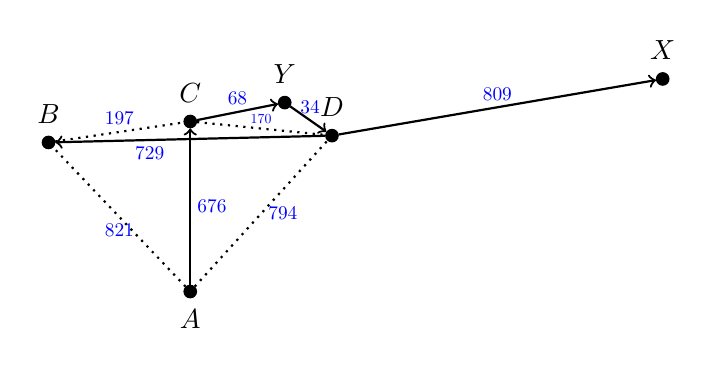
\begin{tikzpicture}[scale=.6]
% \draw[rounded corners=5mm, fill=gray!20, draw=white] (-.7,-.2) -- (3.5,0.7) -- (0.2,4.5) -- cycle;
%  \node[label={[gray]$T_{i_1/i}$}] (Ti1i) at (2,2) {}; 
  \begin{scope}[every node/.style={circle,draw=black,fill= black,minimum size=3.5pt, inner sep=1.6}];
  \node[label=below:$A$] (A) at (0,3) {};
  \node[label=$B$,below] (B) at (-3,6.3) {};
  \node[label=$C$] (C) at (0,6.6) {};
  \node[label=$D$] (D) at (3,6.3) {};
  \node[label=$X$] (X) at (10,7.5) {};
  \node[label=$Y$] (Y) at (2,7) {};
  \end{scope}
	\draw[thick,->] (A) -- (C) node[pos=0.5, right, scale=0.7] {\textcolor{blue}{676}}; 
	\draw[thick,->] (C) -- (Y) node[pos=0.5, above, scale=0.7] {\textcolor{blue}{68}};
	\draw[thick,->] (Y) -- (D) node[pos=0.55,above, scale=0.7] {\textcolor{blue}{34}}; 
	\draw[thick,->] (D) -- (B) node[pos=0.65,below, scale=0.7] {\textcolor{blue}{729}};
	\draw[thick,->] (D) -- (X) node[pos=0.5,above, scale=0.7] {\textcolor{blue}{809}};
	\draw[thick,dotted] (A) -- (D) node[pos=0.5,right, scale=0.7] {\textcolor{blue}{794}};
	\draw[thick,dotted] (A) -- (B) node[pos=0.5,below, scale=0.7] {\textcolor{blue}{821}};
	\draw[thick,dotted] (B) -- (C) node[pos=0.5,above, scale=0.7] {\textcolor{blue}{197}};
	\draw[thick,dotted] (C) -- (D) node[pos=0.5,above, scale=0.5] {\textcolor{blue}{170}};
%	\pic [draw=blue, <->, text=blue,"$\alpha$",angle eccentricity=0.9,left] {angle = D--A--B};
%	\pic [draw=blue, <->, text=blue,"$\beta$",angle eccentricity=0.9,above,left] {angle = A--B--C};
%	\pic [draw=blue, <->, text=blue,"$\gamma$",angle eccentricity=0.9, right] {angle = B--C--D};
%	\pic [draw=blue, <->, text=blue,"$\delta$",angle eccentricity=0.9,right, above] {angle = C--D--A};
%	\pic [draw=blue, <->, text=blue,"$\eta$",angle eccentricity=0.9,right, above, scale=1.4] {angle = C--A--B};
  \end{tikzpicture}
  \end{document}
